% Well-motivated project with success criteria well-justified.

\label{sec:1}
Visual Simultaneous Localization and Mapping (visual SLAM) serves as the foundation of countless modern technologies, with self-driving cars, augmented reality devices, and autonomous drones just being a few examples. By using purely visual inputs, visual SLAM is able to create a 3D map of the surroundings while also localizing the camera's position within this map in real-time.

Unlike other SLAM systems which may use expensive and heavy sensors such as LIDAR, RGB-Depth cameras, or Radar, visual SLAM only requires the ubiquitous camera sensor, allowing the technology to be used in many commercial applications such as Google's ARCore \autocite{arcore}, Boston Dynamic's GraphNav system used on their robot Spot \autocite{graphnav}, and several models of DJI quadcopters \autocite{zou2019collaborative}, underscoring the practicality of this research field.

\section{Motivation}
\label{sec:motivation}
Multi-robot systems are becoming increasingly common as automation continues to grow across a variety of sectors, including self-driving cars, drone swarms, and warehouse robots. These systems require the agents to understand the world around them as well as their peers' locations within that world. This task is typically achieved through technologies such as GPS or motion capture setups, however, not all environments have access to these systems. A few emerging examples include: \noparskip
\smallbreak
{
    \begin{itemize}[nosep]
        \item Search and rescue operations in large indoor environments, assisted by drone swarms.
        \item Self-driving cars in underground road networks.
        \item Multi-agent extraterrestrial exploration.
    \end{itemize}
}

These are scenarios where multi-agent SLAM provides a compelling solution, it allows for mapping unfamiliar environments while maintaining awareness of the positions of all agents involved. However, many of the existing multi-agent visual SLAM implementations are centralized systems, requiring agents to maintain a reliable communication link with a central server in order to operate. This is severely disadvantageous, as environments lacking access to GPS or motion capture systems often also suffer from unreliable communication channels – greatly limiting the use cases of these centralized multi-agent SLAM systems.

Naturally, this leaves us with distributed multi-agent visual SLAM systems that do not rely on a central management server, allowing the agents to be deployed in environments where network infrastructure may be lacking. Instead of utilizing a central node, the agents communicate peer-to-peer when they come within close proximity to one another.

It is easy to see the broad-reaching use cases of such a system. Agents will be able to explore sections of their world independently, or in small teams, sharing new world locations with their peers as they come into communication range using an ad-hoc network. Additionally, agents will be able to accurately determine their peers' locations when they are within communication range, allowing for collision avoidance and cooperative path planning.

\section{Project Overview}
\label{sec:project-overview}
In this project, I: \noparskip
{
    \begin{enumerate}
        \item Design and implement a novel distributed monocular visual SLAM system, capable of localization, relative pose estimation, and collaborative mapping, all while being tolerant to degraded network conditions and not reliant on any single leader agent (\autoref{sec:slam-system}).
        \item Evaluate the performance of my system on standard datasets, \textbf{demonstrating its superior performance over comparable state-of-the-art systems} (\autoref{sec:comparison-to-related-work}).
        \item Create a simulation environment for testing and evaluating my system locally (\autoref{sec:simulation-environment}).
        \item Develop a custom collision avoidance framework (\autoref{sec:motion-controller}) and deploy it alongside my SLAM system on physical robots, \textbf{demonstrating the practical use cases of my system and benchmarking real-world performance} (\autoref{sec:real-world-experiments}).
        \item \textbf{Contribute as a co-author to the paper \textit{The Cambridge RoboMaster: An Agile Multi-Robot Research Platform} \autocite{blumenkamp2024cambridge}}. My distributed SLAM system is included in the paper and used to evaluate the robotics platform (\autoref{sec:cambridge-robomaster-platform}).
        \item Develop \textit{Multi-Agent EVO} – the first open-source evaluation library for multi-agent SLAM systems (\autoref{sec:multi-agent-evo}).
        \item Develop the \textit{Raspberry Pi Video Publisher} – a performant platform for SLAM data collection and augmented reality visualizations – and set up a continuous integration and deployment pipeline to automatically deploy the latest builds to the devices (\autoref{sec:raspberry-pi-video-publisher}).
    \end{enumerate}
}

\begin{leftbar}
    A short video demonstration of my project is provided at the following URL:\\ \url{https://cam-diss.s3.amazonaws.com/video.mp4}\captionbreak Due to the highly visual and 3D nature of my project, \textbf{I strongly recommend viewing the video}. It will provide an intuition of my system, making the following chapters easier to visualize and understand. Additionally, it is referenced throughout this dissertation.
\end{leftbar}

\begin{figure}[h]
    \centering
    \captionsetup{format=plain, labelformat=empty, font=normalsize}
    \begin{subfigure}[t]{0.475\linewidth}
        \centering
        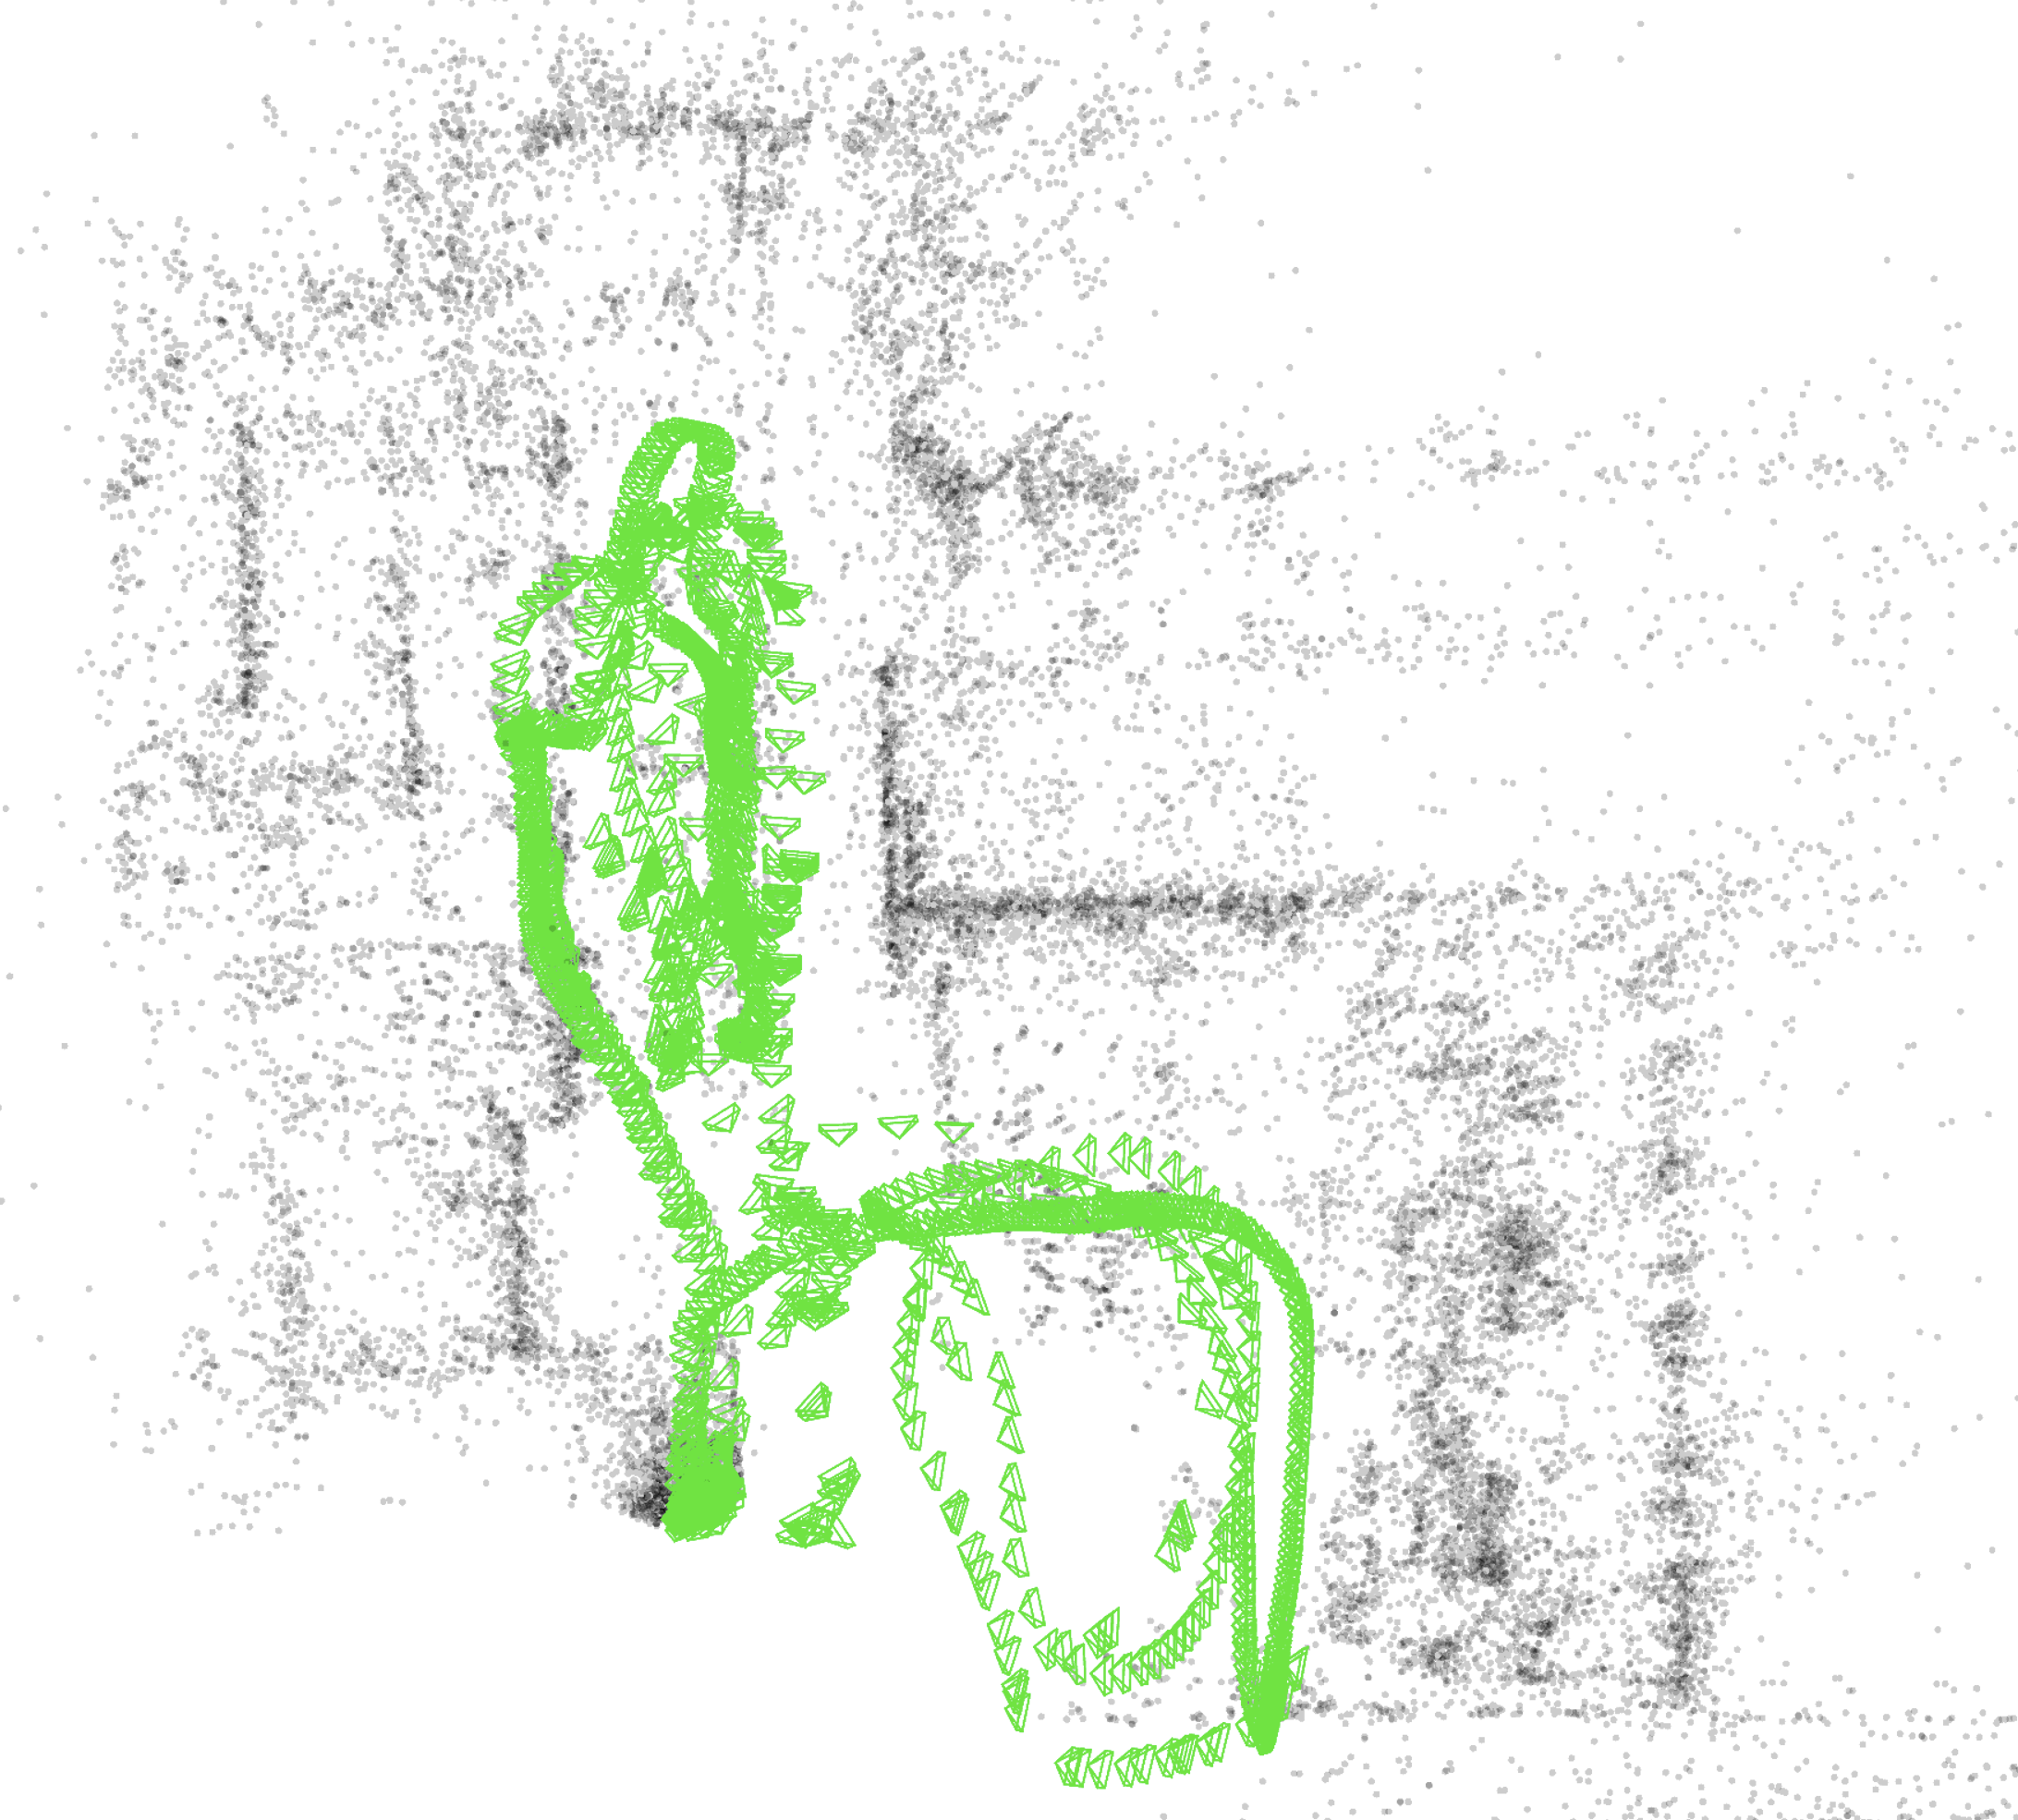
\includegraphics[height=2.3in]{figures/euroc_mh_map.png}
        \caption{EuRoC Machine Hall 01-03}
    \end{subfigure}\hfill%
    ~
    \begin{subfigure}[t]{0.475\linewidth}
        \centering
        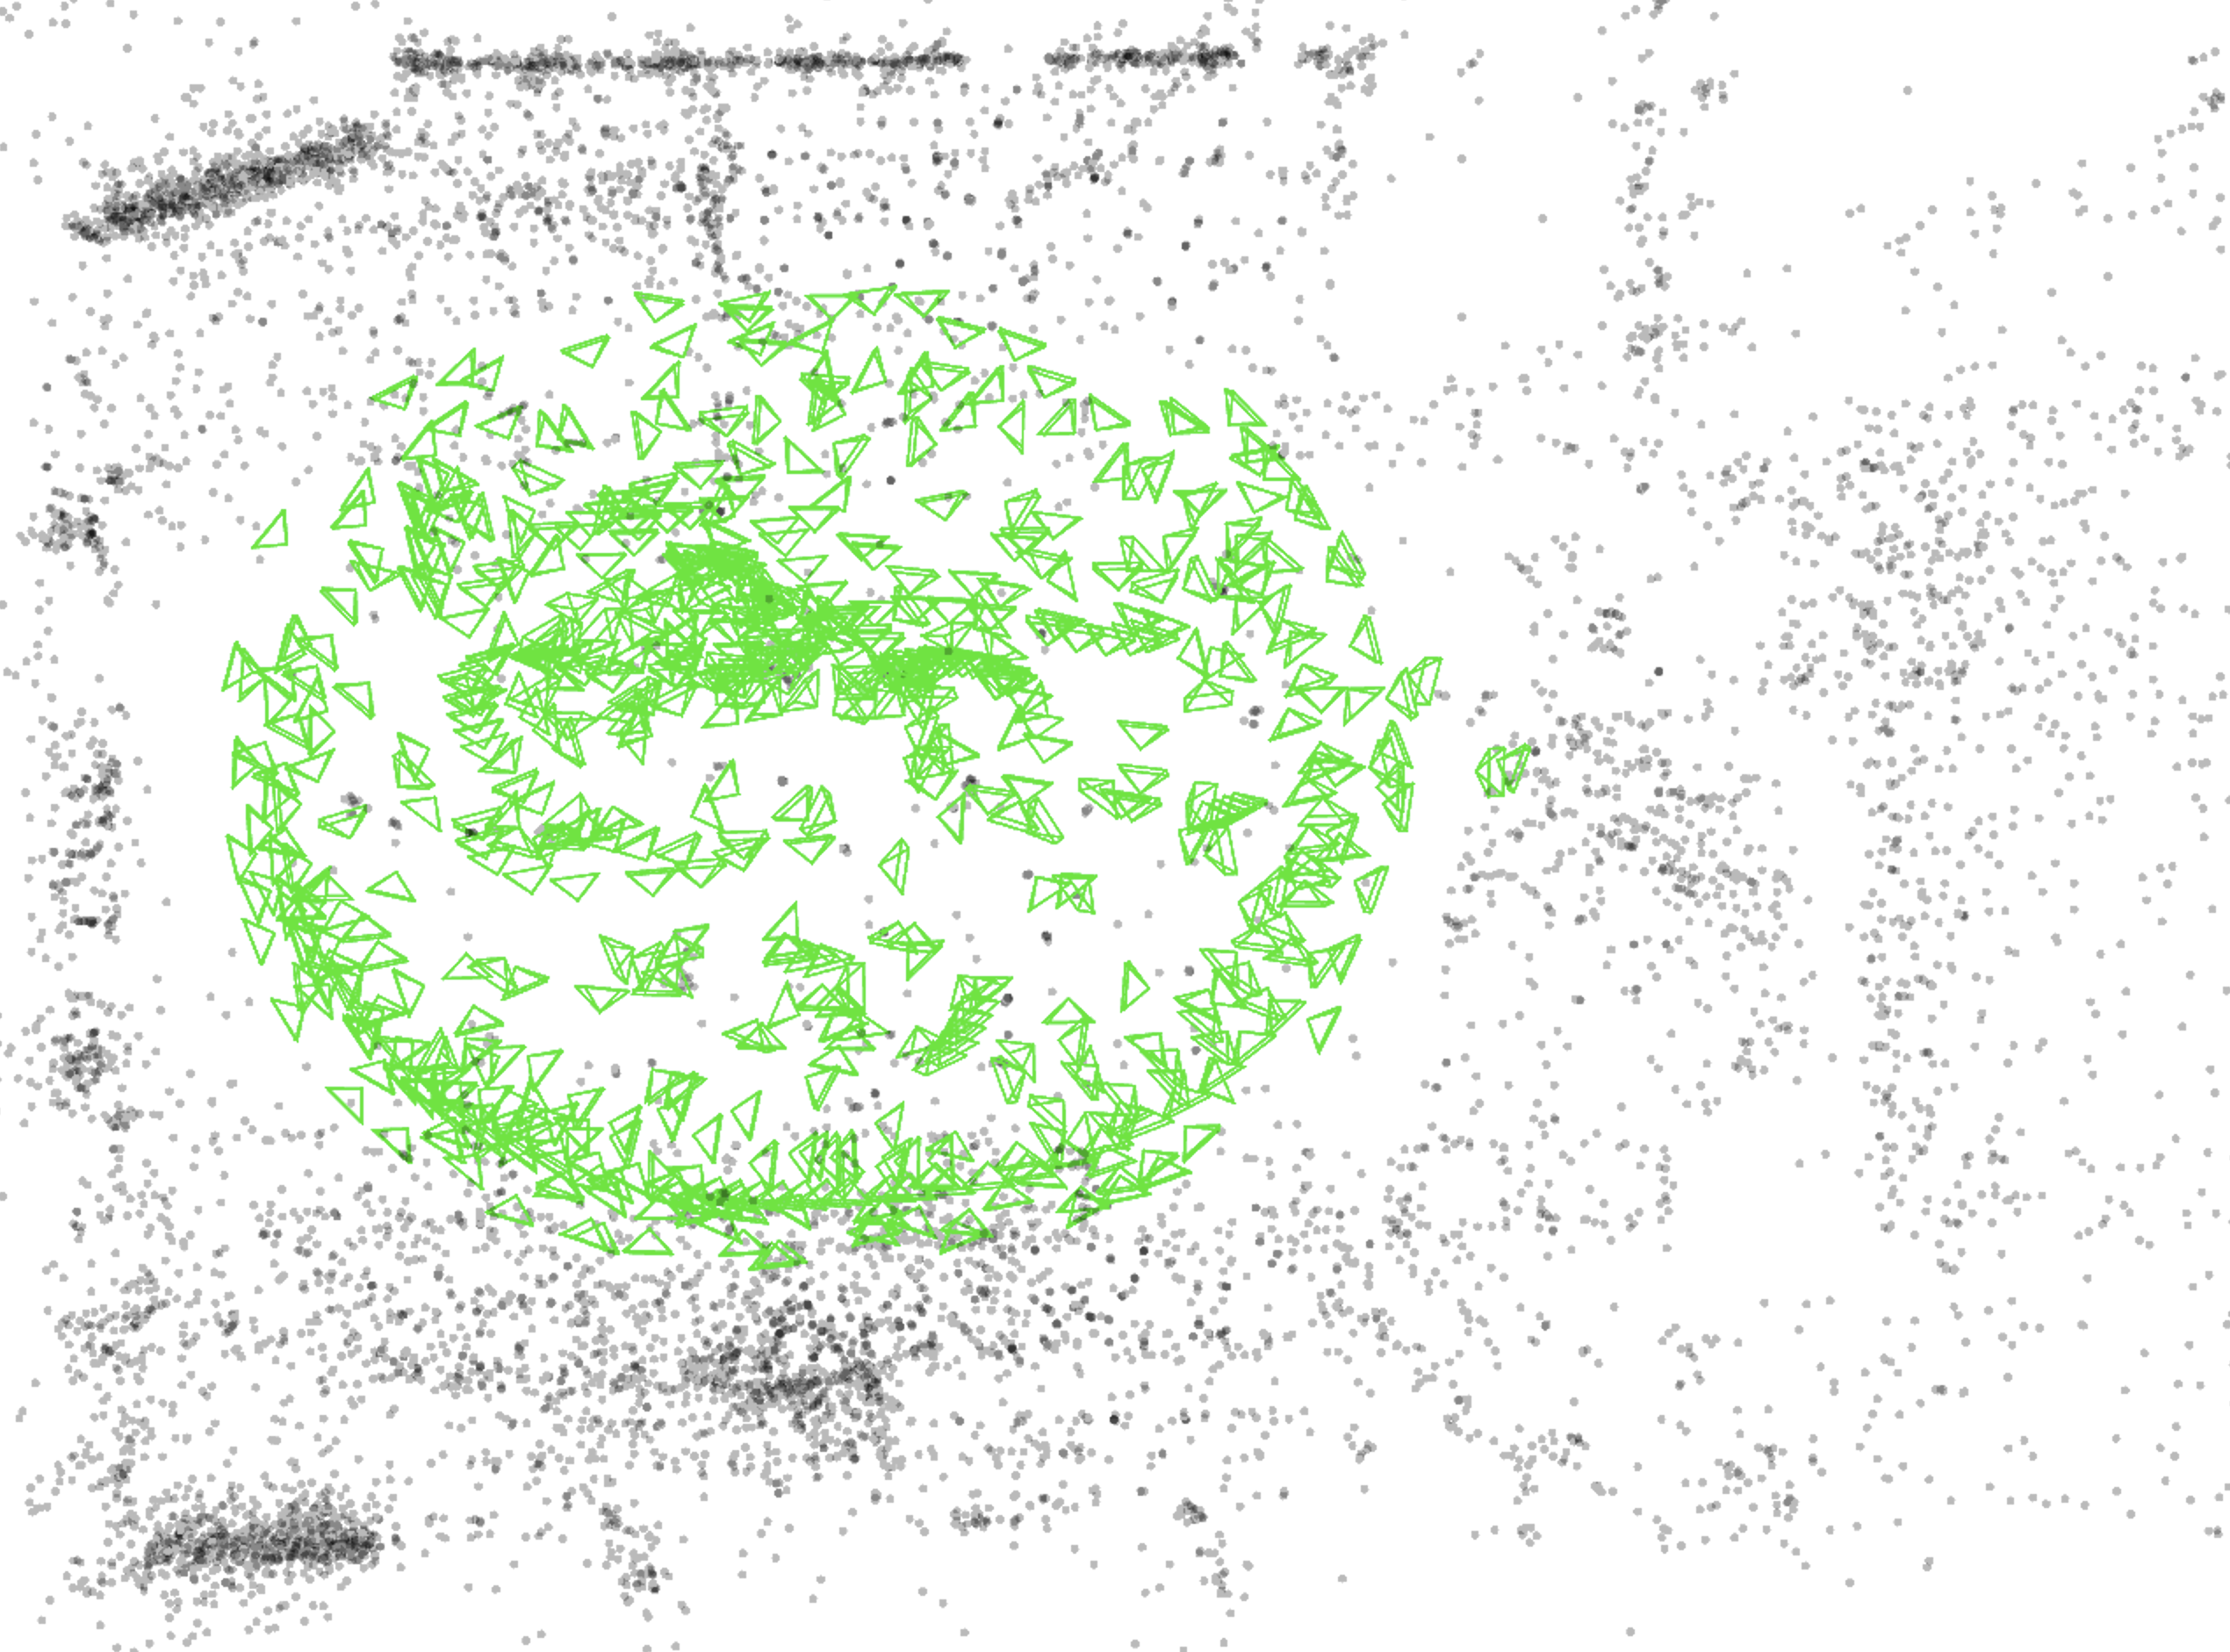
\includegraphics[height=2.2in]{figures/tum_room_map.png}
        \caption{TUM-VI Rooms 1-3}
    \end{subfigure}

    \caption{The figures above display the maps collaboratively built by my distributed SLAM system using only monocular videos from industry-standard multi-agent datasets.}
    \label{fig:example-maps}
\end{figure}
